% Weaknesses of this chapter include mentions of high-bandwidth system that is not actually ever used. The same can be said for the experimental chapter which discusses its design somewhat.

\documentclass[a4paper]{article}
\usepackage{import}
\subimport{../}{preamble}
\begin{document}

\section{Experimental Measurements of Dynamic Tip Dimers}

% Setup procedure
Dynamic interactions and separation-dependent phenomena between two tips are spectroscopically studied using an axial scanning approach. Tips are coupled with another tip in order to maximise optical accessibility to the gap. Although not representing the typical geometry used in TENOM this presents a more optimal geometry to explore plasmonic coupling on a more fundamental level.
Tips are first aligned into the dimer configuration under the supercontinuum laser beam using the capacitive technique described in chapter~\ref{sec:tip_alignment}. Alignment takes place with the laser illumination on to prevent spatial changes to the tip apices, caused by thermal expansion, from occurring post-alignment when spectroscopy is performed.%
\footnote{This behaviour was briefly looked at, with laser-induced cantilever deflection being measured in tips. This suggested that the heat of the focus was causing mechanical deforming or bending of the AFM probe, moving the lateral position of the tip apex and misaligning the tip dimer prior to gap coupling experiments.}
The tip of the stiffer cantilever of the pair is partially positioned in the laser spot and the tip of the softer cantilever is resonantly driven and used as the alignment probe, beginning at distances outside of the laser focus. Sufficient space is left after placement of the stationary tip to accommodate both tip apices equally under the laser spot once brought together. This level of positioning is subjective, with scattering intensity used to estimate an acceptable position for the stationary tip within the collection spot. Once alignment is complete the separation between tips is reduced from around $\sim$\SI{300}{nm} to geometrical contact whilst undergoing measurement.

% Sample preparation
The tips used in experiments, whether commercial or fabricated in-house, are required to have clean metallic surfaces when studying gap plasmon interactions. Layers of insulating surface molecules prevent the gap from narrowing sufficiently to enter the quantum regime, therefore any layers deposited as either a byproduct of a chemical reaction or from carbon deposition in SEM need to be removed. This is done through either plasma cleaning or piranha treatment. To maintain cleanliness some experiments are performed in a nitrogen flow environment.

\begin{figure}[bt]
\vspace{-10pt}
\centering
\fontsize{10pt}{1em}\selectfont
\begin{tikzpicture}
\node [below right] at (0,0)
{\def\svgwidth{0.7\textwidth}
\subimport{./figures/}{simple_optics_dimer_layout.pdf_tex}};
\node [below right] at (5,-2.4)
{\def\svgwidth{0.4\textwidth}
\subimport{./figures/}{tip_dimer_diagram.pdf_tex}};
\end{tikzpicture}
\caption[Experiment configuration for axial tip scanning]{\textbf{Experiment configuration for axial tip scanning.} The laser is centred on the aligned tip dimer for gap spectroscopy. The soft cantilever approaches the stationary, stiff cantilever at a controllable rate $dz$~\si{\nano\metre\per\second}. A bias is applied across the tip junction and the current through the gap is measured. The soft cantilever faces the AFM module for force measurement via cantilever deflection.
A diagram of tip dimer characteristics is shown as an inset. The diagram specifically shows the case for a spherical Au tip dimer, showing the antenna plasmon modes which couple together. Plasmonic coupling depends on both the gap size, $d$, and the particle radius, $R$. The illumination and collection angles, defining $\vec{k}_{\mathrm{incident}}$ and $\vec{k}_{\mathrm{col}}$, are $\theta_{\mathrm{incident}} = \sin^{-1}(0.6-0.8\NA)$ and $\theta_{\mathrm{col}} < \sin^{-1}(0.6\NA)$.
}
\label{fig:simple_optics_dimer_layout}
\vspace{-5pt}
\end{figure}

% Procedure
During scanning measurements on tip dimers, the stationary tip acts as the optical probe, staying fixed in the collection spot throughout the scan, whilst the other tip approaches at a rate of 0.1--\SI{1}{\nano\metre\per\second}. Approach speeds are continually adjusted and optimised during scanning to reduce the time interval between completion of alignment and achieving geometrical contact and minimise any potential lateral drift. Use of a stiffer cantilever ensures that the AFM tip remains fixed in its current position under the laser spot, even once under pressure from the opposite tip. Measurements of the optical scattering, electronic conductance and applied force are taken at each point in the scan. The geometry of this experiment is shown in \autoref{fig:simple_optics_dimer_layout}.
% Optics
The approaching tip perturbs the near-field and interacts with the probe tip. Separation-dependent optical scattering is then collected through the objective collection aperture. Strong scattering of the intense supercontinuum source means 10--\SI{20}{ms} integration times are sufficient for a high quality signal to noise, therefore spectra acquisition does not affect the scan speed. % Not mentioning polarisation sensitivity?
Only light polarised along the tip dimer axis is reported in the context of this work in order to focus on the influence of charge transfer on coupled gap plasmons. % although the rig is capable of measuring in the other polarisation

Simultaneous measurement of gap conductance and applied force supplement optical scattering measurements, enabling correlations to be made between characteristic gap properties to better interpret the relationship between charge transfer and plasmonic coupling.%
\footnote{Each measurement is ran in parallel using multiprocessing in the experiment control method, with each taking a fixed amount of acquisition time. Multiprocessing not only allows data to be acquired around the same time but also decreases the overall measurement time.}
% Electronics
Electronic properties are probed by driving with a d.c.\ voltage and measuring the current through the tip junction to determine its conductance. A bias of \SI{50}{mV} is almost always used to achieve good signal quality in both low-bandwidth and high-bandwidth conductance measurements and to prevent spikes in the noise from setting off the high-bandwidth trigger. Larger voltages increase the electrostatic pull between tips, visible in force measurements, and the resulting high current upon contact would damage tips if not for the current limiting resistor. The smallest current range is fixed at \SI{10}{nA}, with a sensitivity of \SI{10}{fA}, since lesser ranges require longer settling times, slowing the scan rate. At \SI{50}{mV} the smallest measurable conductance is around \num{e-7}\G0.

% Force
The applied force is measured using optical detection of cantilever deflection by the AFM module. At each step in the scan the position of the returning laser beam is averaged for \SI{100}{ms} to determine the mean cantilever deflection, and therefore the mean applied force, over the duration of electronics and optics measurements.
% Summary
Using this combination of measurements allows for a more informed interpretation of nanoscale gap behaviour than by measuring only the optical scattering, as was done originally \cite{savage2012}.

\subsection{Non-Optical Properties of a Nano-Tip Dimer Gap}

Before studying the optical properties of nano-gaps it is beneficial to understand the range of physical phenomena that exist on each characteristic length scale present during scans that traverse from $\sim$\SI{100}{nm} to \SI{0.1}{nm}. With tips well separated, only the separation and optical scattering are meaningful physical quantities. The optical scattering, if plasmonic in origin, is subject to a separation-dependent capacitive interaction. There is no current and no applied force until the separation reduces to below \orderof{\SI{10}{nm}}. Below this point both the current and the force become instrumental in understanding the optical response. Due to the maturity of AFM, STM and molecular electronics there is already a wealth of information explaining both electronic effects and the forces expected on these length scales.

\begin{figure}[bt]
\centering
\includegraphics{figures/tip_scanning_properties}
\caption[Axial force and conductance measurements of a sharp Au tip dimer approaching into contact]{\textbf{Axial force and conductance measurements of a sharp Au tip dimer approaching into contact.} The characteristic AFM snap-in effect is seen in the axial force (a) as a discontinuous jump before the linear application of force in a soft contact regime. The tip apices snap together, reducing the separation to on the order of \SI{1}{nm}, leading to the onset of quantum tunnelling, and finally conductive contact, upon further decreasing the gap separation (b). Dashed and dotted lines are added as guides to the eye showing different features in the scan, such as snap-in and conductance behaviour.}
\label{fig:tip_scan_props}
\end{figure}

\figurename~\ref{fig:tip_scan_props} shows the conductance and axial force measurements from a typical scan once separation has passed below \SI{10}{nm}. The force shows no features until there is a fast negative (attractive) jump in the applied force, showing that the tip has been pulled towards the opposing tip (\figurename~\ref{fig:tip_scan_props}a). This is the signature of water in gap. The lack of a tunnelling current at this point shows that tips must still be separated by more than \SI{1}{nm}. The actual extent of these snaps varies between scans depending on a number of factors, including the humidity, with some scans snapping in closer than \SI{1}{nm}.

% Snap-in
Since experiments are carried out in ambient conditions the surfaces of tips will always be coated in a thin film of water or nanobubbles. Even in a nitrogen environment, its presence is only reduced and not completely removed. When two surfaces come into close proximity a water meniscus forms between them, leading to strong capillary forces \cite{gan2009atomic}. Hence, when the separation between the two tips reduces past the point of meniscus formation they are quickly pulled together \cite{holmberg2003}. This is known in AFM as the ``snap-in" or ``snap-into-contact" and occurs on separations $\sim$5--\SI{30}{nm} \cite{holmberg2003, song2014}. In the above scan the snap distance can be inferred from the displacement required to remove the applied force as \SI{6}{nm}.

To prevent snap-in either a stiffer cantilever must be used (normally in tapping mode) \cite{zhong1993fractured} or the water meniscus has to be removed, which is usually achieved through liquid immersion AFM \cite{hansma1994tapping, putman1994tapping, song2014} or by using plasma treatment to remove hydrophobic contamination \cite{song2014}. In this instance, however, the water layer is advantageous. The presence of the meniscus prevents immediate electrical and geometrical contact and holds tips around \SI{1}{nm} apart until further force is applied. Approach of the tips then occurs in much finer increments due to mechanical resistance from the water. This effectively splits a scan into three regimes - one in which the decreasing intertip separation is directly controlled, one after snap-in where cantilever displacement gradually pushes the tip through the water meniscus (soft interaction), and finally one in which force is applied directly to the opposite tip in geometrical contact (hard-wall contact).

The existence of the soft interaction regime enables sub-nm gaps to be studied with some degree of control since only a fraction of the applied cantilever displacement corresponds to a displacement at the apex. Instead, the meniscus is loaded with an applied force, leading to the linear reverse deflection observed in AFM force measurements. This can be seen in \autoref{fig:tip_scan_props}a where \SI{15}{nm} of cantilever displacement moves the apex $\sim$0.8--\SI{0.9}{nm} (deduced from electron tunnelling measurements). The remaining \SI{14.2}{nm} loads the gap with \SI{8}{nN} of force, proportional to the cantilever's spring constant.

Use of soft AFM probes (contact mode cantilevers) means a greater spatial resolution in the sub-nm regime since force is applied more gently with cantilever displacement.%
\footnote{Smaller $k$ means larger $x$ required for $F=kx$ to meet the same target value.}
Softer cantilevers are also advantageous during tip alignment as they have larger oscillation amplitudes, and therefore lower voltages are needed to reach acceptable signal quality, and also lower bandwidth requirements (\SI{13}{kHz} as opposed to 190--\SI{300}{kHz}).
For these reasons, along with those directly related to tip alignment capabilities (outlined in chapter~\ref{sec:tip_alignment}), one tip in the dimer is usually a contact mode probe while the other tip, which must remain stationary under an applied force, is a stiffer tapping mode probe. Early experiments exclusively used contact mode cantilevers until determining that spectral changes could not be guaranteed to originate from the gap under the application of a large force.

% Electronics
Despite their usefulness in showing the relative motion of the tip, force measurements are somewhat limited in their information on the absolute separation. An estimate of the absolute separation is made possible by studying charge transfer in the gap. Electron tunnelling is the dominant charge transfer mechanism, occurring prior to conductive contact with the current due to tunnelling follows an approximately exponential decay with increasing separation. The conductance in STM is often stated to drop by approximately a factor 10 for every \SI{1}{\angstrom} away from conductive (approximately geometrical) contact. This relation permits deduction of the gap separation to a certain degree using the order of magnitude of the gap conductance.

% Charge transfer
Upon reducing the gap to below \SI{1}{nm} electron tunnelling becomes detectable. Though the absolute value of the conductance for a given separation depends on the gap morphology the relative exponential conductance drop from geometrical contact still approximately holds for $d>\SI{2}{\angstrom}$ \cite{esteban2015}. This makes electron tunnelling a useful method for estimating the gap size to within $\sim$\SI{0.1}{nm}. Once the separation is greater than \SI{1}{nm} the conductance drops to below around \num{e-9}\G0 and the corresponding current becomes difficult to measure without significantly raising the d.c.\ bias. For example, use of a \SI{50}{mV} bias means a current on the order of \SI{1}{fA}, which remains below the currently achievable noise level.

\autoref{fig:tip_scan_props}b shows a typical conductance trace on approach. Once the separation decreases below \SI{1}{nm} the conductance steadily increases with force from \num{e-7} to around \num{e-4}\G0 as the tips transition through the soft interaction regime. At \num{e-4}\G0, the rate of conductance increase slows, signifying the compacting of the meniscus into a single monolayer of water, which requires a greater force to displace. At \num{e-2}\G0 the separation is estimated to be similar in size to a single water molecule (\SI{2.75}{\angstrom}), which, when displaced, causes tips to quickly transition into geometrical contact, saturating with a contact conductance around 100\G0. The displacement of this final gap layer and consequent relief of force on the tip is shown by a decrease in the force gradient during the transition into contact.

Each of the electronic and force measurements described in this section are instrumental in discerning the underlying phenomena occurring in sub-nm gaps. These measurements can then be correlated with optical spectra and used to interpret changes to plasmon coupling, especially changes that depend sensitively on gap morphology or dielectric medium. Using this information, more accurate physical models can be developed to further understand the quantum regime of plasmon coupling than what currently exist.

\section{Plasmonic Coupling Between Tips}

%\begin{figure}[bt]
%\centering
%\def\svgwidth{0.5\textwidth}
%\subimport{./figures/}{tip_dimer_diagram.pdf_tex}
%\caption[Diagram of tip dimer characteristics]{\textbf{Diagram of tip dimer characteristics.} The diagram specifically shows the case for a spherical Au tip dimer, showing the antenna plasmon modes which couple together. Plasmonic coupling depends on both the gap size, $d$, and the particle radius, $R$, where the mobile tip particle approaches a stationary spherical tip at a rate $dz$. The illumination and collection angles, defining $\vec{k}_{\mathrm{incident}}$ and $\vec{k}_{\mathrm{col}}$, are $\theta_{\mathrm{incident}} = \sin^{-1}(0.6-0.8\NA)$ and $\theta_{\mathrm{col}} < \sin^{-1}(0.6\NA)$.}
%\label{fig:tip_dimer_diagram}
%\end{figure}

Plasmonic interactions between tips are studied using the dimer approach. Two AFM tips are dynamically brought together to form a single gap structure, mimicking a plasmonic dimer cavity, whilst the optical scattering, conductance and force are simultaneously measured. The resulting experiment geometry is shown as an inset in \autoref{fig:simple_optics_dimer_layout}. Both sharp and spherical Au tips are studied in a range of dimer permutations, in order to understand how plasmons in each tip couple. This is also compared with results from hyperspectral characterisation, indicating whether plasmons initially exist in such structures.

\subsection{Sharp Tip Dimer Interactions}

% Experimental data
\begin{figure}[bt]
\centering
\includegraphics{figures/sharp_au_tip_dimer_scan}
\caption[Spectra of a sharp Au tip approaching a stationary sharp Au tip]{\textbf{Spectra of a sharp Au tip approaching a stationary sharp Au tip.} Sharp Au tips are BudgetSensors GB series AFM probes. There are no identifiable plasmon resonances initially in the system and no new modes appear with decreasing gap size. The lack of any shifting suggests that plasmons are not present in the system. The increase in intensity and its spectral shape are an artefact of adding more of the reflective tip facet into the confocal collection aperture.}
\label{fig:sharp_tip_scan}
\end{figure}

The first combination of AFM tips studied is a sharp Au tip interacting with another sharp Au tip. Hyperspectral characterisation indicates that sharp Au tips lack any observable LSPs. Similarly for dimer experiments, no observable coupling is expected despite the possibility that gap modes may exist. Reducing the separation between two sharp Au tips indeed shows no resonances or coupled modes (\autoref{fig:sharp_tip_scan}). Scattering increases are seen, however these do not shift with decreased separation or change with conductance. They are instead attributed to more of the reflective tip facet entering the confocal collection aperture as the tip is approached to the stationary tip. Spectral scattering increases also bear resemblance to the spectral density of the illumination and intensity changes correlate well with changes in the torsional force, further supporting this claim.

Tunnelling currents are observed to have no effect on scattering from the gap, despite reports suggesting that tunnelling electrons excite plasmons \cite{lambe1976, berndt1991, bharadwaj2011, wang2011, divitt2013, ye2014}. The reason for this is the small \SI{50}{mV} bias. The excitation condition $\hbar\omega<eV$ is not satisfied for visible frequencies and hence only low energy SPPs in the IR could be excited.%
\footnote{For a \SI{50}{mV} voltage the limiting frequency is \SI{7.6e13}{rads}, or $\lambda=\SI{24.8}{\micro\metre}$ deep in the IR.}
Using higher voltages around \SI{2}{V} would give a finite probability that an electron would excite an SPP, with intensity depending on the current through the junction and the collection geometry.%
\footnote{For a \SI{2}{V} voltage the limiting frequency is \SI{3.0e15}{rads}, or $\lambda=\SI{630}{nm}$. Hence plasmons can be excited in the red frequencies of the visible spectrum and below.}
In the current geometry only localised gap modes could be observed since the system lacks a means of measuring SPP leakage radiation. Furthermore, reports detecting radiation from localised gap modes have used sensitive CCDs with long integrations. Hence, within this system when using \SI{10}{ms} integration times, it is unlikely that tunnelling-induced radiation will be detected.

The conclusions drawn from these experiments agree with those of individual sharp Au tip spectroscopy. Sharp Au tips do not show any evidence of supporting plasmons which readily couple with light and there have been no detected signatures of plasmon coupling between similar tips. However, both the gap geometry and previous spectroscopic (spectroscopy, TERS and electrical excitation) measurements on tips suggest that plasmons and gap modes can exist in such geometries. It can only be stated that, based on the measurements shown here, only radiative antenna-like plasmons can be seen in the far-field and that tips are not capable of supporting these. Further tests outside the scope of the work discussed in this thesis would be required to test for SPP excitation and how these effect the underlying mechanisms of TENOM.

In order to optically probe plasmon coupling in a sub-nm cavity between two tips, a tip geometry which couples with far-field light is required. Sharp Au tips are clearly inadequate for this purpose. For this reason the spherical tip geometry, with its visible wavelength plasmon resonances, facilitates the dynamic study of plasmonic coupling in nanoscopic gaps.

\subsection{Spherical Tip Dimer Interactions}

By using spherical Au tips the tip-tip system mimics the prototypical spherical AuNP dimer. It is through this  arrangement that a controllable plasmonic dimer is recreated. The presence of radiative plasmons, discussed in chapter~\ref{ch:tip_plasmonics}, enables the detection of gap modes as tips transition from the non-interacting regime at $\sim$\SI{300}{nm} through into the charge transfer regime before entering conductive contact. By utilising such a controllable plasmonic system, plasmon coupling can be better understood on a fundamental level and unravel the remaining questions regarding plasmonics in sub-nm gaps.

\subsubsection{Spherical Tip Interactions with a Spherical Tip}

\begin{figure}[bt]
\centering
\begin{tikzpicture}
\node [below left] at (0,0) {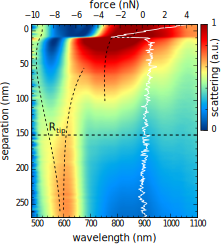
\includegraphics{figures/classical_tip_dimer_1}};
\node [below right] at (0,0) {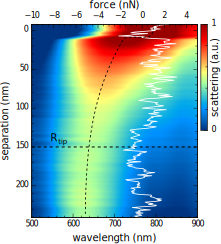
\includegraphics{figures/classical_tip_dimer_2}};
\node [below left] at (-6.6,0) {\textbf{a}};
\node [below right] at (0,0) {\textbf{b}};
\end{tikzpicture}
\caption[Spectra of a spherical Au tip approaching a stationary spherical Au tip]{\textbf{Spectra of a spherical Au tip approaching a stationary spherical Au tip.} Spherical Au tips are Au-coated NanoTools B150 AFM probes. Two scans are presented in the classical interaction regime, showing similar phenomena. The separation is estimated based on known tip displacements to the point of snap-in. Guides to the eye are added to highlight mode behaviour. Horizontal dashed lines indicate the radius separation, at which point coupling is expected to begin. In both cases, but more clear in (b) with tips having similar initial LSPs, bonding hybridised modes form, which redshift with decreasing intertip separation (increasing coupling). With slightly dissimilar initial LSPs anti-bonding hybridisation can be seen as a blueshifting mode with decreasing intertip separation.}
\label{fig:spherical_tip_dimer_scan}
\end{figure}

The first configuration of spherical tips studied is that of a spherical Au tip approaching another spherical Au tip. In this instance the 600--\SI{650}{nm} LSPs of the individual tips interact and form observable gap modes. Representative scans of two approaching spherical Au tips are shown in \autoref{fig:spherical_tip_dimer_scan}, in which plasmon resonances are dynamically followed from non-interacting to classically coupled. It should be noted that in previous microscope designs the short-range tip alignment meant that plasmons were only seen once in a coupled state near \SI{750}{nm} \cite{savage2012}. Improvements to the range of the tip alignment technique using optical detection have allowed the full range of plasmon coupling to be studied.

Coupling between spherical tips appears very similar to that of a large nanoparticle dimer. Plasmons are initially uncoupled and only the single LSP of the probed tip is observed. Plasmons begin to interact at $d \approx R_{\mathrm{tip}} = \SI{150}{nm}$ as is classically expected, where $d$ is estimated based on the point of snap-in. As the gap width decreases the individual plasmon modes increasingly couple together, redshifting monotonically and scattering increasingly. The initial plasmon mode at \SI{630}{nm} redshifts to around \SI{800}{nm} in each scan at the point of snap-in, where the separation is reduced to around \SI{1}{nm}. Increased scattering is due to both increasing coupling and an increased amount of scattering metal entering the confocal sampling volume of the objective. Once the gap has decreased sufficiently ($d \ll R_{\mathrm{tip}}$) the confocal collection argument is negligible as the sampling volume becomes saturated, hence all further changes are due to plasmon coupling in the gap.

For large distances the rate of redshift is dominated by the increase in capacitive coupling as the separation decreases. In each scan a large abrupt redshift of the coupled mode correlates with snap-in. The large redshift on snap-in is due in part to two effects: the decrease in separation as the tip is pulled in by capillary forces and the increase in refractive index as the gap constitution transitions from air to water (and any material contained in the water meniscus). The intensity of the lowest order mode begins to decrease once the gap width decreases below \SI{1}{nm}. This effect is attributed to the mode becoming increasingly confined to the point of becoming non-radiative. Similar changes in mode intensity are often seen in classical simulations and occur well before the onset of any significant quantum effects \cite{savage2012, esteban2015}.

%\begin{figure}[bt]
%\centering
%\includegraphics{figures/classical_mode_fits}
%\caption[LSP resonance wavelengths and amplitudes over multiple scans of spherical tip dimers]{\textbf{LSP resonance wavelengths and amplitudes over multiple scans of spherical tip dimers.} The antisymmetric nature of the system mimics a heterodimer leading to the observation of both bonding (red) and anti-bonding (blue) hybridised modes.}
%\label{fig:heterodimer_measurements}
%\end{figure}

Slightly different classical coupling physics is observed when the dimer symmetry is broken. In some cases where initial tip resonances differ by $\sim$\SI{50}{nm} coupling is better described by a heterodimer model rather than a homodimer. Under the asymmetrical condition, anti-bonding modes can be excited due to phase retardation and are no longer dark since dipoles do not exactly cancel. Depending on which particle is probed, either the one supporting the lower or higher energy initial resonance, either a redshifting bonding mode or a blueshifting anti-bonding mode is observed to be the dominant gap resonance (see \figurename~\ref{fig:plasmon_hybridisation} and \cite{nordlander2004}). The tip dimer probed in \autoref{fig:spherical_tip_dimer_scan}a clearly exhibits both mode configurations and is a good representation of what is seen across many additional scans.
%These two types of hybridised modes are additionally seen together across many different scans, for which a subset of resonances traced through measurements prior to snap-in are shown in \autoref{fig:heterodimer_measurements}. The amount of shift visible in the figure depends on the initial resonance position and the separation at which snap-in occurred.

This effect has been documented previously \cite{nordlander2004} but never directly observed dynamically. The anti-bonding configuration is typically non-physical in most plasmonic systems since both particles are driven with the same phase of light. However, with larger particles, such as these \SI{150}{nm} radius spherical Au tips, the phase symmetry is broken allowing anti-bonding hybridised plasmons to be excited. Both the blueshift and the later redshift at small separations are found in spherical tip scans, indicating the interaction and anti-crossing between the lower order anti-bonding mode and the higher order, adjacent bonding mode. The higher order bonding modes responsible for this are then seen after snap-in.

\subsubsection{Spherical Tip Interactions with a Sharp Tip}

\begin{figure}[b]
\centering
\includegraphics{figures/sharp-AuNP_tip_dimer}
\caption[Spectra of a spherical Au tip approaching a stationary sharp Au tip]{\textbf{Spectra of a spherical Au tip approaching a stationary sharp Au tip.} No coupling phenomena are observed due to the mismatch between plasmon modes.}
\label{fig:spherical_sharp_tip_scan}
\end{figure}

The interaction between the same spherical Au tip and a sharp Au tip is investigated with results shown in \autoref{fig:spherical_sharp_tip_scan}. Despite the sharp tip perturbing the field around the spherical tip, acting as the optical antenna, no changes are observed in the spherical tip plasmon, suggesting that there is no interaction between sharp tips and spherical tip plasmons. This is in agreement with predictions that a sharp tip should not deviate the resonance of a planar surface \cite{downes2006, hugall2012}, for which the much larger tip could be considered. The tip acts as a point perturbation not strong enough to significantly modify the more distributed antenna-like response. This observation also supports the measurements shown in chapter~\ref{sec:tip_applications}, where the laser was assumed to stay on resonance with the AuNP tip as it approached the BTh-coated sharp Au tip.

\end{document}